\setcounter{chapter}{7}
\setchapterabstract{This chapter outlines the application of Article 101 of the Treaty on the Functioning of the European Union (TFEU), which prohibits anti-competitive agreements, decisions, and practices. Article 101(1) lists behaviours that may restrict competition, such as price-fixing, market sharing, and limiting production, while Article 101(3) allows exemptions if agreements create pro-competitive benefits like efficiency gains or improved product quality. These exemptions require that the benefits be passed on to consumers, and that the restrictions are necessary. Restrictions by "object" need no proof of anti-competitive effects, while others require a detailed market impact analysis. The chapter also highlights the "\textit{de minimis}" threshold, block exemptions, and the balance between restrictions and potential benefits under Article 101(3).}
\chapter{Article 101 Prohibition and Exemption}
\vspace{-1.5cm}

{\chaptoc\noindent\begin{minipage}[inner sep=0,outer sep=0]{0.9\linewidth}\section*{Framework}\end{minipage}}

    \begin{enumerate}
        \item Arrangements that do not fall under the first paragraph of Article 101 TFEU.
    
            \(\Rightarrow\) \textbf{Lawful}
        
        \item Arrangements that fall under the first paragraph \textit{and} at the same time fall under the third paragraph.
    
            \(\Rightarrow\) \textbf{Lawful}: Reg. 1/2003, Article 1(2): arrangements caught by Article 101(1) which satisfy the 4 conditions of Article 101(3) shall not be prohibited, no prior decision to that effect being required.
        
        \item Agreements that fall under the first paragraph but do not meet the conditions laid down in the third paragraph.
    
            \(\Rightarrow\) \textbf{Unlawful}: therefore, prohibited and void
    \end{enumerate}

\section*{Article 101(1) of the TfUE}

    Agreements, Decisions, Concerted practices, which have as their object or effect the prevention, restriction or distortion of competition within the internal market, and in particular those which:

        \begin{enumerate}
            \item Fix purchase or selling prices or any other trading conditions;
            \item Limit or control production, markets, technical development, or investment;
            \item Share market or sources of supply;
            \item Apply dissimilar conditions to equivalent transactions with other trading parties, thereby placing them at a competitive disadvantage;
            \item Make the conclusion of contracts subject to the acceptance by other parties of supplementary obligations which, by their nature or according to commercial usage, have no connection with the subject of such contracts.
        \end{enumerate}

        \Remark{
        The list of agreements that may be caught by the prohibition is illustrative, not exhaustive.
        }

\section{Preliminary remarks}

    \begin{enumerate}[label=\alph*.]
        \item A contractual restriction of the freedom to act involving two (or more) parties does not necessarily result in a restriction of competition.
        
        To understand whether an agreement restricts competition, we need economic analysis. Apart from a small class of agreements that are considered to have as their object a restriction of competition, in all other situations enforcers should demonstrate that there is substantial competitive harm to show that there has been an infringement of Article 101.
        
        \item No “rubber stamp” analysis. Every case deserves full demonstration of the ``capability'' of an arrangement to harm consumers (or, better, practices that may worsen market well-functioning as a result of consumer surplus reductions) to be caught under Article 101. Very time-consuming.
        
        \item The first passage of the analysis consists in finding the relevant markets. In theory, this step is not necessary if it is possible, even without its delimitation, to show that an agreement restricts competition. This happens when the object of an agreement is clearly anti-competitive (restriction by object).
        
        \item Article 101 covers both horizontal and vertical agreements, even if these latter ones are generally considered less damaging to competition than horizontal agreements.
        
        \item More in general, you can ideally put different types of agreements on a line and distinguish them according to the intrinsic degree of restrictiveness (their nature).
    
        \[
        0 \quad \text{---------------------------------------------->} \quad 1
        \]
    
        Some agreements do not cause any harm while others are “restrictive by nature.” According to the theory of collusion, at the very right end of the spectrum, you find cartels that not only fix quantities or prices but also provide monitoring schemes to implement the illegal plan and measures to punish non-compliance (need to avoid cheating ex ante and to effectively punish cheaters ex post).
    \end{enumerate}

\newpage
    \subsection{Definition of object – ratio of the prohibition}

        These two requirements are \textbf{alternative}, not \textbf{cumulative}: These two words are to be read disjunctively.
        
        \begin{itemize}
            \item[i.] If the object is clearly anti-competitive, there is no \textbf{NEED} to prove that it also produced anti-competitive effect to apply art. 101(1)
            \item[ii.] Only when it is not clear that the object of an agreement is to restrict competition, it is thus necessary to consider whether it might have the effect of doing so.
        \end{itemize}
        
        From (i) it can be derived that it is of paramount importance to understand the meaning of “object”\sn{\Definition{
        Object means the objective of the agreement, i.e. the meaning and purpose of the agreement considered in the economic context in which it is to be applied
        }{Object}} and which types of practices can be put in the “object box”.

        There is no role for subjective intention of the parties, i.e. if when entering the agreement, they wanted and/or they knew they would have adopted an agreement clearly anti-competitive. Those agreements must be prohibited because they have such a likely potential to have negative effects that it is redundant to prove that they also had actual effect on the market.

        The very likely anticompetitive potential is mainly due to: 
        \begin{enumerate}[label=(\alph*)]
            \item The very serious nature of the restriction, and
            \item Prior experience (case law, but also economic analysis) showing that such restrictions are likely to produce negative effects on the market and to jeopardise the objectives pursued by the EU competition rules.
        \end{enumerate}
        
        \textbf{Administrative efficiency criterion}: it is a waste of public resources to spend time to demonstrate something that is already evident; \textit{AG Kokott in T-Mobile}: the classification of certain types of agreement as restrictive by object “sensibly conserve resources of competition authorities and the justice system”.
        
        Furthermore, the existence of a well defined category of restriction forbidden by object “creates legal certainty and allows all market participants to adapt their conduct accordingly”. It is a clarifying guideline for undertakings, but if the indication is wrong the risk is that of \textbf{overdeterrence} or \textbf{underdeterrence}.

    \subsection{How to determine a restriction by object}

        Very different messages over time, also from the ECJ. Very recently: ECJ, C-298/22, \textit{BPN/BIC Português SA}, 29 July 2024:

        The restriction by object concept should be interpreted narrowly, i.e. refers only to coordination that reveals a sufficient degree of harm on competition. Certain types of coordination between undertakings can be regarded, by their very nature, as being harmful to the proper function of competition and markets.
        
        \Remark{\textbf{HOW?} To determine whether an arrangement can be a restriction by object, it is necessary to examine:
        \begin{enumerate}[label=\alph*.]
            \item The content of that agreement, decision or practice,
            \item The economic and legal context of which it forms a part, and
            \item Its objectives.
        \end{enumerate}}

    \begin{enumerate}[label=\alph*.]
        \item “In order to examine the content of the agreement, it is necessary to examine its various aspects in order to determine whether the collusion in question has characteristics enabling it to be linked to a form of coordination between undertakings which must be regarded, by its very nature, as harmful to the proper functioning of normal competition, which is in particular the case if any coordination exhibiting such characteristics is, precisely because of those characteristics, capable of creating conditions of competition which do not correspond to the normal conditions of the market in question.”

        \item As regards the economic and legal context of the agreement at issue, since the concept of restriction by object refers only to agreements that must be regarded, by nature, as harmful to the proper functioning of normal competition, it in no way requires that the effects of that agreement, decision or practice on competition, be they actual or potential, or negative or positive, be examined or, a fortiori, proven. However, that does not preclude the need to take into consideration the nature of the goods or services concerned, as well as the real conditions of the structure and functioning of the sectors or markets in question.

        Therefore, the examination of the economic and legal context of those forms of coordination must make it possible to ascertain whether, where a form of agreement is harmful to competition only in certain circumstances relating, in particular, to the nature of the goods or services at issue, to the real conditions of the functioning of the market and to its structure, those circumstances exist. The purpose of taking the context into account is thus to ascertain that no particular circumstance surrounding the agreement, decision or concerted practice at issue is such as to rebut the presumption that the form of coordination to which it belongs is harmful to competition.

        \item Lastly, as regards the aims pursued by the agreement at issue, it is necessary to determine the objectives which that agreement, decision or practice is intended to achieve from a competition standpoint. Nevertheless, the fact that the undertakings involved acted without having a subjective intention to prevent, restrict or distort competition and the fact that they pursued certain legitimate objectives are not decisive for the purposes of the application of Article 101(1) TFEU.
        
        An examination of all those factors must, in any event, show the precise reasons why the agreement, decision by an association of undertakings or concerted practice at issue reveals a sufficient degree of harm to competition such as to justify a finding that that agreement has as its object the prevention, restriction or distortion of competition.
        
        \Example{
        “an exchange of information which, although not formally presented as pursuing an anticompetitive object, cannot, in the light of its form and the context in which it occurred, be explained other than by the pursuit of an objective contrary to one of the constituent elements of the principle of free competition must be regarded as constituting a restriction by object.”
        }
        
    \end{enumerate}

\newpage
    \subsection{The Object Box}

        However, in practice we use the \textbf{object box}.

        \begin{enumerate}[label=\alph*.]
            \item It is for the Court of Justice to determine which agreements should be allocated to the object box. We use case law.
            \item The box is not sealed with scotch tape. Over time, some agreements may fall in the box, while others come out of it, e.g.: maximum RPM.
        \end{enumerate}

        \Example{
        \textbf{HORIZONTAL AGREEMENTS}, i.e. to:
            \begin{itemize}
                \item Fix prices (and price components, costs, etc.)
                \item Exchange information on future prices which reduces uncertainty about future behaviour
                \item Share markets, clients, outlets, quotas
                \item Limit output, including the removal of excess capacity
                \item Limit sales
                \item Perform collective exclusive dealing schemes (collective boycott)
                \item Adopt pay for delay strategies (pay competitors to delay the launch of competing products)
                \item Spread misleading information?
            \end{itemize}
        }

        \Example{
        \textbf{VERTICAL AGREEMENTS}, i.e. to:
            \begin{itemize}
                \item Impose fixed or minimum resale prices
                \item Impose export bans
            \end{itemize}
        }
            
        

        \subsubsection{How to determine a (new kind of) restriction by object}

            When an arrangement is not already in the box:

            \begin{enumerate}[label=\alph*.]
                \item In view of the requirement to interpret the concept of restriction of competition by object restrictively, although practices for which there are no precedents may be regarded as restrictions by object, that classification should be restricted to cases where the anticompetitive nature of an agreement or practice is obvious or where the practices in question have no credible explanation other than to restrict competition on the market.
                \item \textbf{Preamble}: La Roche and Novartis colluded to exclude the cheap drug Avastin, used in the treatment of the most common eyesight condition in the elderly as well as other serious sight problems, and channel demand towards the much more expensive drug Lucentis, through an artificial distinction between the two products.
            \end{enumerate}

            The analysis leads to the conclusion that:
            \begin{quote}
                “an arrangement put in place between 2 undertakings marketing 2 competing products, which concerns the dissemination, in a context of scientific uncertainty, to the regulatory authority, healthcare professionals, and the general public of misleading information relating to adverse reactions resulting from the use of one of those products for the treatment of diseases not covered by the marketing authorisation for that product, with a view to reducing the competitive pressure resulting from such use on the use of the other medicinal product, constitutes a restriction of competition \textit{by object} for the purposes of that provision.”
            \end{quote}

            \Example{
            Lucentis has a market authorisation for glaucoma and its price is 800 €; \\ Avastin has no market authorisation for that disease but it is known that it can be used as a substitute of Lucentis because its composition is exactly the same. Its price is 80 €.
            }

\section{Effect}

    Only where it is not possible to find a restriction by object, in order to determine whether a certain agreement may be caught by the Article 101(1) prohibition, it is necessary to conduct an extensive analysis of its effects on the market (EUCJ 21 December 2023, \textit{International Skating Union v Commission}, C-124/21 P, § 99).

    In \textit{Brasserie de Haecht v. Wilkin}, the CJEU held that an agreement “cannot be examined in isolation from the earlier context, that is, from the factual and legal circumstances causing it to prevent, restrict or distort competition.”
    
    In order for an agreement to be deemed a restriction of competition by effect, the EC looks at the actual conditions in which it functions, in particular:
    \begin{enumerate}[label=\roman*.]
        \item the economic context in which the undertakings operate;
        \item the products/services covered; and
        \item the structure of the market.
    \end{enumerate}

    \subsection{The need of a Theory of Harm}

        \textbf{EU Guidelines on the application of Article 101(3)}

        “Account must be taken of both actual and potential effects. In other words, the agreement must have likely anti-competitive effects, which is up to the Commission to demonstrate (in the case of restrictions of competition by effect there is no presumption of anti-competitive effects).
        
        To be restrictive by effect, an agreement must affect competition to such an extent that on the relevant market, negative effects on prices, output, innovation, or the variety or quality of goods and services can be shown or at least expected with a reasonable degree of likelihood.
        
        The prohibition of Article 101 only applies where, on the basis of proper market analysis, it can be concluded that the agreement has very likely significant anti-competitive effects on the market.”

    \subsection{Empirical analysis and the counterfactual}

        The CJUE ruled that restrictive effects must be demonstrated by empirical facts. Anticompetitive effects must therefore be supported not only by:
        \begin{enumerate}[label=\Roman*.]
            \item a theory of harm, but also by
            \item robust empirical analysis.
        \end{enumerate}
        
        \textbf{How?}
        
        In determining whether an agreement has a restrictive effect on competition, it is necessary to consider what the position would have been in the absence of the agreement.
        
        We need to establish a counterfactual: by comparing two different situations, it is possible to form a view as to whether the agreement could have the effect of restricting competition (or have actually restricted competition).
        
        \subsubsection{Appreciability}

        An agreement which has as its object or effect a restriction of competition is to be considered automatically prohibited?

        \begin{itemize}
            \item EC Commission in the first 1960s: every restriction of competition is prohibited (to avoid prohibition and voidness, the 4 conditions laid down by Art. 101(3) should have been satisfied).
            \item 1969: The ECJ ruled in \textit{Volk v. Vervaecke} (1969) that if the undertakings concerned lacked market power, the agreement would fall outside Art. 101:
            
            “an agreement falls outside the prohibition in Art. 101 when it has only an insignificant effect on the markets, taking into account the weak position which the persons concerned have on the market of the product in question.”

            \item Further evolution:
                \begin{itemize}
                    \item \textbf{Restrictions by object} must always be considered significant, or appreciable, and thus prohibited according to Art. 101. EUCJ clarified that an agreement which has as its object the restriction of competition within the internal market “constitutes, by its nature and independently of any concrete effects that it may have, an appreciable restriction of competition” (EUCJ, Expedia).
                    \item \textbf{Restrictions by effect} must be analysed on a “case by case” basis. However, for legal certainty and simplification, the EC Commission issued a “de minimis”\sn{\Note{i.e., concerning agreements of minor importance.}}
                \end{itemize}
        \end{itemize}

\newpage
    \subsection{Commission’s translation of “Weak Position” - The \textit{de minimis} doctrine}

        \Remark{This is not valud for \textbf{by object restrictions.}}

            Restrictions of competition by effect are not appreciable if:
            \begin{enumerate}[label=\alph*.]
                \item The aggregate market share held by the parties to the agreement is ≤ 10\% on any of the relevant markets affected (agreements between horizontal competitors); or
                \item The market share held by each of the parties to the agreement is ≤ 15\% on any of the relevant markets affected, where the agreement is made between undertakings which are not actual or potential competitors on any of those markets (agreements between vertical competitors or non-competitors).
                \item Where competition is restricted by the cumulative effect of agreements entered by different suppliers or distributors (cumulative foreclosure effect), the market share thresholds are reduced to 5\%. A cumulative foreclosure effect is unlikely to exist if less than 30\% of the relevant market is covered by parallel (networks of) agreements having similar effects.
            \end{enumerate}
            
            \textbf{This is an important safe harbour} \(\rightarrow\) wiping out most potentially restrictive agreements between EU undertakings.\sn{\Note{These are guidelines, i.e. soft law: for the principle of legitimate expectation they must be followed by the Commission, but not by the EU Courts, National Courts, National Competition Authorities. However, they are – at least – taken into consideration by these latter bodies.}}

            Thus, appreciability can be seen as a combination of:
            \begin{enumerate}[label=\Alph*.]
                \item The nature of the agreement (ideally here you measure the “degree of intrinsic restrictiveness of an agreement”);
                \item Market power of the parties concerned (de minimis notice);
                \item Combined cumulative (network) effects, and other market characteristics.
            \end{enumerate}
            
            The more restrictive the agreement, the less market power is needed in order to trigger the Article 101(1) prohibition (and vice versa)\sn{\Note{Remember, however, that agreements may always be tested also under Article 101(3).}}.
            
\section{Article 101(3) - The four conditions }

    An agreement that falls within Art. 101(1) is not necessarily unlawful (and void). Art. 101(3) provides a “legal exception” to the prohibition in Art. 101(1) by providing that it may be declared inapplicable in respect of arrangements that satisfy cumulatively 4 conditions:

    \textbf{Two positive conditions:}
    \begin{enumerate}[label=\arabic*.]
        \item The agreement must contribute to improving the production or distribution of goods or to promoting technical and economic progress;
        \item The agreement must transfer to consumers a fair share of the resulting benefit.
    \end{enumerate}
    
    \textbf{Two negative conditions:}
    \begin{enumerate}[label=\arabic*.]
        \setcounter{enumi}{2}
        \item The agreement must not impose unnecessary restrictions;
        \item The agreement must not eliminate competition.
    \end{enumerate}
    
    The Commission has issued Guidelines to interpret these four conditions.
    
\section{Exemptions}

        \subsubsection{1. When}

            Remember that we have an \textbf{ex-post enforcement system} for agreements. Thus, it is for the plaintiff or the NCA or the EU Commission to show that the agreement is caught by Article 101(1). If they succeed, then it will be for the defendant to show that the arrangement satisfies all the conditions set down by Article 101(3). Article 101(3) is a \textbf{DEFENCE}.

            See Article 2, Reg. 1/2003 - \textit{Burden of proof}.
            
            \begin{quote}
            “In any national or Community proceedings for the application of Articles (101) and (102) of the Treaty, the burden of proving an infringement of Article 101(1) or of Article 102 of the Treaty shall rest on the party or the authority alleging the infringement. The undertaking or association of undertakings claiming the benefit of Article 101(3) of the Treaty shall bear the burden of proving that the conditions of that paragraph are fulfilled.”
            \end{quote}

        \subsubsection{2. Which}

            Any type of agreement can be defended under Art. 101(3). The ECJ ruled that an undertaking can assert the applicability of the exception provided for in Art. 101(3) “in all circumstances”.

            Thus, also restrictions by object can be, at least in theory, exempted. De facto impossible for cartels, but not for any kind of price fixing:
            
            In \textit{Visa Int. - Multilateral Interchange Fee} (2002), the Commission granted an exemption to a MIF\sn{\Note{MIF is the fee that the acquiring bank (that is, the bank which contracts merchants for Visa card acceptance) pays to the issuing bank (that is, the bank which issues Visa cards to consumers) as a reimbursement for each transaction with a Visa card.}} agreed between acquiring and issuing banks within the Visa system:
            \begin{quote}
            “it is not the case that an agreement concerning prices is always to be classified as a cartel (…). Furthermore, a MIF is not a price charged to a consumer, but a remuneration paid between banks who must deal with each other for the settlement of a card payment transaction and thus have no choice of partner. The absence of some sort of default rule on the terms of settlement could lead to abuse by the issuing bank, which is in a position of monopsony as regards the acquiring bank for the settlement of an individual payment transaction. Thus, some kind of default arrangement is necessary, but the question of whether it qualifies for exemption or not will depend on the details of the arrangement.”
            \end{quote}

        \subsubsection{3. How}

            The benefit produced by an agreement must be something of objective value to the EU as whole, not a private benefit to the parties themselves. Those benefits must be balanced against the restrictions of competition. Obviously, an exemption is possible IFF the advantages claimed of the agreement outweigh the detriments it might produce.

        \subsubsection{4. Robust Evidence}

            The parties must produce \textit{“a detailed, robust and compelling analysis that relies in its assumptions and deductions on empirical data and facts”}. The more serious is the restriction of competition, the stronger must be the evidence of the benefits generated by the agreement.

        \subsubsection{5. What}

            \textbf{Narrow or broad view of Art. 101(3)?} Do we have to consider only efficiency gains, or can we also take into consideration other factors (EU Treaty most important goals, the need to protect industrial sectors – and their workforce – hit by general or specific crisis, our personal data, etc.)?

            Art. 101(3) is also applied by NCAs and national judges…. Thus, it’s easier and safer to take a narrower view (efficiencies, and other goals only to corroborate the conclusion; other goals can be pursued differently, e.g., by regulation: exception, sustainability).
            
            \textit{EC Commission’s Guidelines} (written in the “more-economic-approach” era):
            \begin{quote}
            “Agreements that restrict competition may at the same time have pro-competitive effects by way of efficiency gains. Efficiencies may create additional value by lowering the cost of producing an output, improving the quality of the product or creating a new product. When the pro-competitive effects of an agreement outweigh its anti-competitive effects, the agreement is on balance pro-competitive and compatible with the objectives of the Community competition rules. The net effect of such agreements is to promote the very essence of the competitive process, namely, to win customers by offering better products or better prices than those offered by rivals.”
            \end{quote}

            \Remark{From 2023-24: There is an explicit exception for sustainability goals}

        \subsubsection{General principles}

            According to the Commission, goals pursued by other Treaty provisions can be considered ONLY to the extent that they can be subsumed under the four conditions of Art. 101(3). Thus, other EU Treaties’ goals can support the Commission’s antitrust decision, when it is not clear whether Eff. > Rest. (like in \textit{Ford/Volkswagen} or \textit{Philips/Osram}).

            \begin{quote}
                The Union shall establish an internal market. It shall work for the sustainable development of Europe based on balanced economic growth and price stability, a highly competitive social market economy, aiming at full employment and social progress, and a high level of protection and improvement of the quality of the environment. It shall promote scientific and technological advance.
            \end{quote}

            \begin{table}[h!]
            \centering
            \begin{tabular}{|>{\raggedright\arraybackslash}m{6cm}|>{\centering\arraybackslash}m{3cm}|}
            \hline
            \textbf{Competitive balancing according to the EC Commission} & \textbf{Balance} \\ \hline
            Restrictions of competition (Article 101(1)) & -- \\ \hline
            Efficiencies (Article 101(3)) & + \\ \hline
            Other EC Treaties' Goals (Article 101(3)) & Yes, \textit{ad adiuvandum} \\ \hline
            Non-EC Treaties' Goals & NO (still? A lot of discussion on sustainability) \\ \hline
            \end{tabular}
            \caption{Competitive balancing by the EC Commission}
            \end{table}

    \subsection{Efficiencies as a defence}

        All efficiency claims must be substantiated in order to verify:

        \begin{enumerate}[label=\alph*.]
            \item The nature of the claimed efficiencies, so that it would be possible to verify that they are objective in nature. Cost savings that arise from the mere exercise of market power cannot be taken into account. For example, reduced competition may lead to lower sales and marketing expenditures, as a consequence of the reduction in output and value. These cost reductions do not produce any pro-competitive effects on the market: they merely allow the undertakings concerned to increase their profits and are therefore irrelevant from the point of view of Art. 101(3).

            Furthermore, the Guidelines draw a distinction between:
            \begin{itemize}
                \item \textbf{Cost efficiencies} (development of new production methods and technologies; integration of existing assets, economies of scale and scope, better planning of production, reduction in the cost of raw materials, components, etc.)
                \item \textbf{Qualitative efficiencies} (R\&D agreements; distribution agreements with pre or post-sales services)
            \end{itemize}
            
            \item  The link between the agreement and the efficiencies should be direct. A direct causal link exists for instance where:
                \begin{itemize}
                    \item A technology transfer agreement allows the licensees to produce new or improved products, or
                    \item A distribution agreement allows products to be distributed at lower cost or valuable pre/post-sale services to be provided.
                \end{itemize}
            
            An example of an indirect effect would be a case where it is claimed that a restrictive agreement allows the undertakings concerned to increase their profits, enabling them to invest more in research and development to the ultimate benefit of consumers (this defense has been used in the pharmaceutical sector). While there may be a link between profitability and R\&D, this link is generally not sufficiently direct to be considered in the context of Art. 101(3).
            
            \item The likelihood and magnitude of each claimed efficiency. In case of efficiencies in the form of new or improved products and other non-cost-based efficiencies, undertakings claiming the benefit of Article 101(3) must describe and explain in detail the nature of the efficiencies and how and why they constitute an objective economic benefit.
            
            They must also describe the method(s) by which the efficiencies have been or will be achieved (for long-term agreements). The data submitted must be verifiable, so that there can be a sufficient degree of certainty that the efficiencies have materialised or are likely to materialise.
            
            \item How and when each claimed efficiency would be achieved. Where the agreement has yet to be fully implemented, the parties must substantiate any projections as to the date from which the efficiencies will become operational so as to have a significant positive impact on the market.
        \end{enumerate}

    \subsection{Fair share for consumers}

        The fair share for consumers condition is a “pass on” requirement to buyers of the product (other firms or consumers) on the relevant market/s.

        \begin{itemize}
            \item Consumers are considered as group/s. Thus, if more groups are affected, each group must be better off.
            \item Some agreements may increase market power and thus prices together with other kinds of benefits to consumers. In that event, those benefits (in terms of quality, quicker development of a new product, etc.) must more than compensate for the potential increase in prices.
            \item The greater the restriction of competition under Art. 101(1), the greater must be the efficiency and the pass-on under Art. 101(3).
            \item When both restriction and pro-competitive effects are substantial, the Commission must consider that rivalry and competitive pressure are important long-term drivers of efficiency and innovation (thus, in case of doubt, it is better to stop than to allow an agreement which strongly increases market power: \textit{Fribourg defeats Chicago}!).
        \end{itemize}
        
        \textbf{Cost efficiencies}: especially with variable cost reduction, pass-on benefits to consumers are likely, since pricing and output decisions are determined predominantly by variable costs and demand conditions.
        
        \textbf{Qualitative efficiencies}: very difficult to measure benefits and to balance those benefits in comparison to the negative effects due to an increase in market power. 

        \Remark{However, the Guidelines acknowledge that new and improved products (product innovation) are an important source of consumer welfare.}

    \subsection{Indispensability}

        The agreement must not impose restrictions not indispensable to the attainment of the efficiencies created by the agreement. This condition implies a two-fold test.

        \textbf{First}, the restrictive agreement as such must be reasonably necessary to achieve the efficiencies.  
        \textbf{Second}, individual restrictions of competition flowing from the agreement must also be reasonably necessary for the attainment of the efficiencies.
        
        The decisive factor is whether the restrictive agreement and individual restrictions make it possible to perform the activity in question more efficiently than would likely have been the case in the absence of the agreement or the restriction concerned. The test requires that the efficiencies be specific to the agreement, i.e., that there are no other economically practicable and less restrictive means of achieving these efficiencies\sn{\Note{In making this latter assessment, the Commission must take into account market conditions and business realities facing the parties to the agreement.}}.
        
        A and B combine in a new entity (JV) their respective production technologies to achieve higher output and lower raw material consumption. The JV is granted an exclusive licence to their respective production technologies. The parties transfer their existing production facilities to the JV. They also transfer key staff to ensure that existing learning economies can be exploited and further developed. It is estimated that these economies will reduce production costs by a further 5\%. The output of the JV is sold independently by A and B.
        
        In this case, the indispensability condition needs an assessment of whether the benefits could be substantially achieved by means of, e.g., a mere cross-licence agreement, which would be likely to be less restrictive because A and B would continue to produce independently.  
        \textbf{Answer}: very unlikely, since under a licence agreement the parties would not be able to benefit in the same seamless and continued way from their respective experience in operating the 2 different technologies, resulting in significant learning economies.
        
        Once it is found that the agreement is necessary to produce the efficiencies, the indispensability of each restriction of competition flowing from the agreement must be assessed. In this context, it must be assessed whether individual restrictions are reasonably necessary to produce the efficiencies. The parties to the agreement must demonstrate their claim about both the nature of the restriction and its intensity.
        
        A single restriction is indispensable if its absence would eliminate or significantly reduce the efficiencies arising from the agreement or make it significantly less likely that they will materialise. The assessment of alternative solutions must consider the actual and potential improvement in the field of competition by the elimination of a particular restriction or the application of a less restrictive alternative.

        \Remark{\textbf{Rule of thumb:} The more serious the restraint, the stricter the indispensability test.}

    \subsection{No elimination of competition}

        We are still ordoliberalist. As a general rule: (\textit{Richard Whish})
        
        \begin{itemize}
            \item[a.] the more that competition is already weakened in the market before the agreement, and
            \item[b.] the more that the agreement will further reduce competition in the market \dots
        \end{itemize}
        
        \[
        \Rightarrow
        \]
        
        \begin{itemize}
            \item[c.] the more likely it is that the agreement will be considered to eliminate competition substantially.
        \end{itemize}

\newpage
    \subsection{Block Exemptions}

        Article 101(3) provides that the prohibition of Article 101(1) could be declared inapplicable both in relation to agreements and to categories of agreements. The Treaty thus envisages not only (ex post) individual assessments, but also more general provisions aimed at regulating categories of agreements.

        Block Exemption Regulations (BER) are very useful because they grant an automatic exemption and then a sort of automatic “safe harbour” for specific contracts/agreements.
        
        \textbf{A)} An agreement complying with a block exemption regulation cannot be declared invalid by a national court or by a National Competition Authority.
        
        \textbf{B)} If an agreement complies with a “BER,” it is valid not only for the past, but also for the future! (for all the duration of the regulation). 
        
        Thus, BERs are very important (and appreciated) for legal certainty.
        
        BERs have a standardized form. They specify:
        \begin{itemize}
            \item A number of clauses that must not be included if an agreement is to enjoy the block exemption (hardcore restrictions); e.g., for R\&D: a limitation on output and sales; the fixing of prices when selling the products or licensing the technologies to third parties; a restriction of territories to which, or the customers to whom, the parties may passively sell the products or licence the technologies.
            \item Thresholds in terms of market shares (e.g., for vertical agreements, the cap is 30\%; for R\&D 25\%, etc.).
            \item Some exceptions.
            \item The Commission’s power to withdraw the benefit of a block exemption (for the future) where it finds that a particular agreement (covered by a block exemption regulation) has effects which are incompatible with Article 101(3).
        \end{itemize}
        
        The duration is usually specified in the regulation and/or linked to the expiry date of the block exemption regulation.
        
        \textbf{Vertical Block Exemptions:}
        \begin{itemize}
            \item Regulation 720/2022 on vertical agreements;
            \item Regulation 461/2010 on vertical agreements relating to the motor vehicle aftermarket;
            \item Regulation 316/2014 on tech transfer agreements.
        \end{itemize}
        
        \textbf{Horizontal Block Exemptions:}
        \begin{itemize}
            \item Regulation 1217/2010 on R\&D;
            \item Regulation 1218/2010 on specialisation agreements;
            \item Many other regulations covering specific industries and sectors (transport and shipping).
        \end{itemize}

\newpage
        \subsubsection{The Relationship between safe harbours, prohibitions and exemptions}

            \textbf{A)} A restriction (other than an object restriction) is not caught by Article 101(1) if it falls under the thresholds specified by the De Minimis Notice.
            \begin{itemize}
                \item \textbf{However}, the fact that an agreement does not fall under the De Minimis thresholds does not mean that it is automatically prohibited by Article 101(1).
            \end{itemize}

            \noindent
            \textbf{B)} An agreement that satisfies the conditions laid down in a Block Exemption Regulation (BER) is considered lawful under Article 101.
            \begin{itemize}
                \item \textbf{However}, the fact that an agreement does not fall under the market share thresholds specified in a certain BER does not mean that it is not eligible for an individual exemption. To be sure, it does not mean that the agreement must be prohibited under Article 101, either.
            \end{itemize}
            
            The De Minimis Notice and BERs = \textbf{“positive” Safe Harbours} that play an important role for legal certainty. Positive (relative and absolute) presumptions of no violation under the thresholds; no presumption of unlawfulness if those thresholds are exceeded.

        
            \begin{figure}[h!]
                \centering
                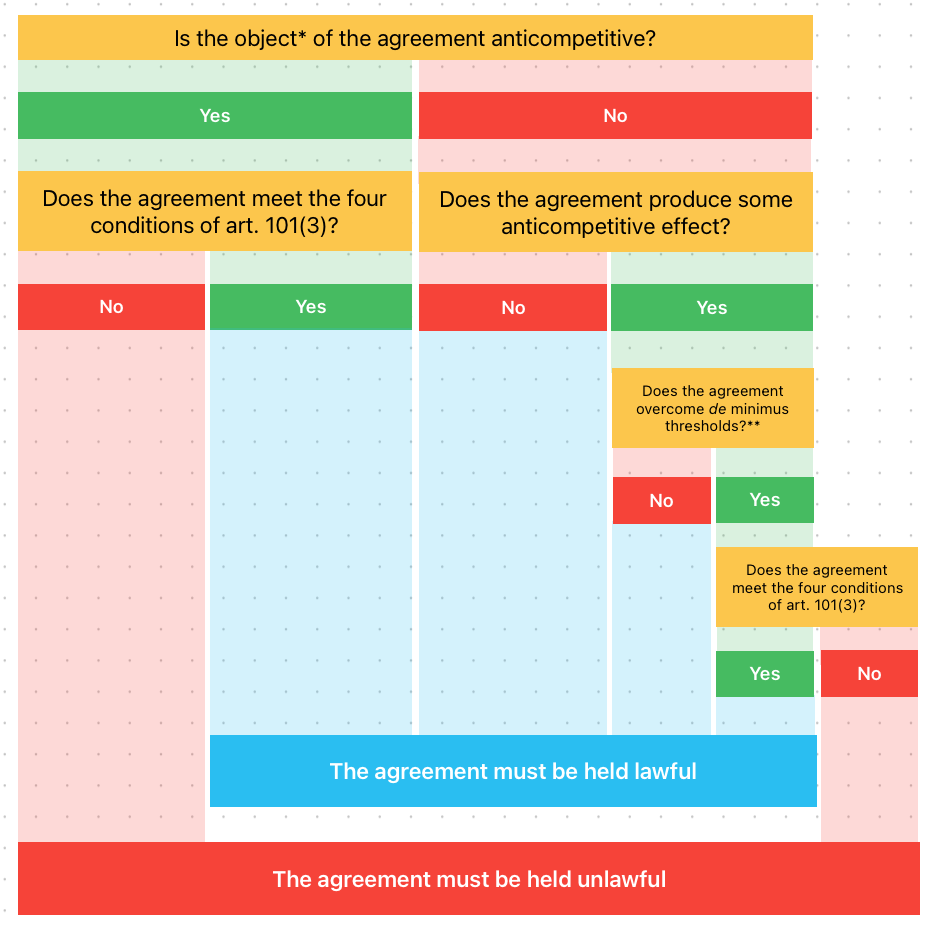
\includegraphics[width=1\linewidth]{final_recap.png}
            \end{figure}